%%% Please replace what is within each curly bracket with the correct information below. %%%
%%% The first field is already filled in for you.  %%%

\def\ClassName {COMP6600} % Your course 


%\solution{
% \fbox{\begin{minipage}[t][5cm][t]{13cm} \Answer \end{minipage}} 
% }
%%%%% FILL IN YOUR ANSWERS TO EACH QUESTION BY REPLACE WHAT IS IN THE CURLY BRACKETS.
\def\Answer{\textbf{Put your answer here:}}
\def\AnswerNoPrompt{}

%%COMMENT OUT TO PRODUCE BLANK DOCUMENT
\def \showSolutions{}

\documentclass[twoside]{article}
\usepackage{placeins}
\usepackage{class}
\usepackage{graphicx}
\graphicspath{{./figs/}}
\usepackage{amsmath, amsthm, amssymb}
\usepackage{url} 
\usepackage{enumerate}
\usepackage{wrapfig}
\usepackage{enumitem}
\usepackage{color}
\usepackage{pifont}
\usepackage{mdwlist}
\usepackage[lofdepth,lotdepth]{subfig}
\usepackage{mdwlist}
\usepackage[ampersand]{easylist}
\usepackage{wasysym}
\usepackage{tikz}

\usetikzlibrary{shapes.geometric}
\usetikzlibrary{positioning}

\ListProperties(Hide=100, Hang=true, Progressive=3ex, Style*=-- ,
Style2*=$\bullet$ ,Style3*=$\circ$ ,Style4*=\tiny$\blacksquare$ )
\title{HW1}
\usepackage{multirow}

\pagestyle{myheadings}

\renewcommand{\P}{\mathbf{P}}
\newcommand{\eat}[1]{\ignorespaces}
\newcommand{\todo}[1]{ {\color{blue} TODO: #1} }
\newcommand{\X}{\ding{110}}
\newcommand{\F}{$\bullet$}
\newcommand{\Pac}{$<$}
\newcommand{\bigCI}{\mathrel{\text{\scalebox{1.07}{$\perp\mkern-10mu\perp$}}}}
\def\truefalse{\vspace{0.3in} \item (\emph{true} or \emph{false}) }
\def\indep{\perp\!\!\!\perp}
\def\sgn{\mathop{\mathrm{sign}}}
\newcommand{\solutionspace}[4]{\fbox{\begin{minipage}[t][#1][t]{#2} \textbf{#3} 

\solution{}{#4} \end{minipage}}}

% Bubbles for multiple choice questions
\newcommand{\emptycircle}{$\Large\bigcirc$}
\newcommand{\filledcircle}{$\Large\newmoon$}
\newcommand{\mcqb}{$\bigcirc$\ \ }
\newcommand{\mcqs}{\solution{\mcqb}{$\Large\newmoon$\ \ }}
\newcommand{\emptysquare}{{\Large $\square$}\ \ }
\newcommand{\filledsquare}{{\Large $\boxtimes$}\ \ }
\newcommand{\squaresolution}{\solution{\emptysquare}{\filledsquare}}


\begin{document}
\thispagestyle{empty}

\def\Name {}  % Your name
\def\AuburnID{} % Your AuburnID

\def\TwoHours{    
    \emptycircle
    % \filledcircle
} 
\def\FourHours{    
    \emptycircle
    % \filledcircle
} 
\def\SixHours{    
    \emptycircle
    % \filledcircle
} 
\def\EightHours{    
    \emptycircle
    % \filledcircle
} 
\def\MoreThanEightHours{    
    \emptycircle
    % \filledcircle
} 


%%%%%%%%%%%%%%%%%%%%%%%%%%%%%%%%%%%%%%%%%%%%%%%%%%%
%%%%%%%%%%%%%%%%%%%% Problem 1 %%%%%%%%%%%%%%%%%%%%
%%%%%%%%%%%%%%%%%%%%%%%%%%%%%%%%%%%%%%%%%%%%%%%%%%%

\def \Oneb{x}
%%%%%%%%%%%%%%%%%%%%%%%%%%%%%%%%%%%%%%%%%%%%%%%%%%%
%%%%%%%%%%%%%%%%%%%% Problem 2 %%%%%%%%%%%%%%%%%%%%
%%%%%%%%%%%%%%%%%%%%%%%%%%%%%%%%%%%%%%%%%%%%%%%%%%%

\def \Twob{x}

%%%%%%%%%%%%%%%%%%%%%%%%%%%%%%%%%%%%%%%%%%%%%%%%%%%
%%%%%%%%%%%%%%%%%%%% Problem 3 %%%%%%%%%%%%%%%%%%%%
%%%%%%%%%%%%%%%%%%%%%%%%%%%%%%%%%%%%%%%%%%%%%%%%%%%
\def \Threea{x}

\def \Threeb{x}

%%%%%%%%%%%%%%%%%%%%%%%%%%%%%%%%%%%%%%%%%%%%%%%%%%%
%%%%%%%%%%%%%%%%%%%% Problem 4 %%%%%%%%%%%%%%%%%%%%
%%%%%%%%%%%%%%%%%%%%%%%%%%%%%%%%%%%%%%%%%%%%%%%%%%%
\def \Foura{x}

\def \Fourb{x}

\def \Fourc{x}

%%%%%%%%%%%%%%%%%%%%%%%%%%%%%%%%%%%%%%%%%%%%%%%%%%%
%%%%%%%%%%%%%%%%%%%% Problem 5 %%%%%%%%%%%%%%%%%%%%
%%%%%%%%%%%%%%%%%%%%%%%%%%%%%%%%%%%%%%%%%%%%%%%%%%%
\def \Fiveai{x}
\def \Fiveaii{x}
\def \Fiveaiii{x}
\def \Fiveaiv{x}


\def \Fivebi{y}
\def \Fivebii{y}
\def \Fivebiii{y}
\def \Fivebiv{y}


\def\Fiveci{y}
\def\Fivecii{y}
\def\Fiveciii{y}
\def\Fiveciv{y}
\def\Fivecv{y}
\def\Fivecvi{y}
\def\Fivecvii{y}
\def\Fivecviii{y}
\def\Fivecix{y}
\def\Fivecx{y}

\def\Fivedi{y}
\def\Fivedii{y}
%%%%%%%%%%%%%%%%%%%%%%%%%%%%%%%%%%%%%%%%%%%%%%%%%%%%%%%%
%%%%%%%%%%%%%%%%%%%% STAFF USE ONLY %%%%%%%%%%%%%%%%%%%%
%%%%%%%%%%%%%%%%%%%%%%%%%%%%%%%%%%%%%%%%%%%%%%%%%%%%%%%%

%% You don't need to fill out the following, only for grading purposes
\def \OneGReason{}
\def \OneHReason{}
\def \OneIReason{}
\def \ThreeCAdmissibleReason{}
\def \ThreeCConsistentReason{}
\def \ThreeDAdmissibleReason{}
\def \ThreeDConsistentReason{}
\def \FourAAReason{}
\def \FourABReason{}
\def \FourACReason{}
\def \FourADReason{}
\def \FourAEReason{}
\def \FourAFReason{}
\def \FourBReason{}

%
%                                  Y\     /Y
%                                  | \ _ / |
%            _____                 | =(_)= |
%        ,-~"     "~-.           ,-~\/^ ^\/~-.
%      ,^ ___     ___ ^.       ,^ ___     ___ ^.
%     / .^   ^. .^   ^. \     / .^   ^. .^   ^. \
%    Y  l    O! l    O!  Y   Y  lo    ! lo    !  Y
%    l_ `.___.' `.___.' _[   l_ `.___.' `.___.' _[
%    l^~"-------------"~^I   l^~"-------------"~^I
%    !\,               ,/!   !                   !
%     \ ~-.,_______,.-~ /     \                 /
%      ^.             .^       ^.             .^  
%        "-.._____.,-"           "-.._____.,-"
%

\maketitle 
\smallskip
\smallskip
\textbf{INSTRUCTIONS}

\begin{itemize}
\item \textbf{Due:} \textbf{Wednesday, 12 February 2025 at 11:59 PM CST.} 
\item \textbf{Format:} Write your answers in the \texttt{yoursolution.tex} file and latex a pdf (preferred) or you can type directly on the blank pdf. Make sure that your answers are within the dedicated regions for each question/part. If you do not follow this format, we may deduct points. 
% You may use digital tools (e.g., an iPad) to handwrite your solutions, but make sure they are legible.
% We reserve the right to take points off if we can't read your solution. 
\item \textbf{Images:} To insert pictures, we recommend drawing it on PowerPoint or Google Drawings, saving it as an image and including it in your latex source.
\item \textbf{How to submit:} Submit a pdf with your answers on Canvas. Log in and click on our class 5600/6600 and click on the submission titled Homework 1 and upload your pdf containing your answers. 
\item \textbf{Policy:} See the course website for homework policies and Academic Integrity.

\end{itemize}

\begin{center}
\begin{tabular}{|r|c|}
\hline
\begin{minipage}{3cm}~\\Name~\\~\\\end{minipage} & \begin{minipage}[c][1cm][c]{8cm} ~ \Name \end{minipage}  \\
\hline
\begin{minipage}{3cm}~\\Auburn ID~\\~\\\end{minipage} & \AuburnID \\
\hline
\begin{minipage}{3cm}~\\Hours to complete? ~\\\end{minipage} & \solution{\emptycircle}{\TwoHours} (0, 2] hours \hspace{0.5cm} \solution{\emptycircle}{\FourHours} (2, 4] hours \hspace{0.5cm}
\solution{\emptycircle}{\SixHours} (4, 6] hours \hspace{0.5cm} \\
&
\solution{\emptycircle}{\EightHours} (6, 8] hours \hspace{0.5cm}
\solution{\emptycircle}{\MoreThanEightHours} $>$ 8 hours \\
\hline

\end{tabular}
\end{center}



\vfill

\smallskip
\smallskip
\smallskip
\smallskip
\smallskip

\begin{center}
{\bf For TA use only}\\
\begin{Large}
\begin{tabular}{|r|r|r|r|r|r|r|r|}
\hline
Q1 & Q2 & Q3 & Q4 & Q5 & Total \\
\hline
\quad/23 &\quad/10 & \quad/25 & \quad/17 &\quad/25 & \quad/100 \\
\hline
\end{tabular}\end{Large}
\end{center}

\newpage
\begin{problem} {Search and Heuristics}

% $\begin{center} \includegraphics[scale=.33]{figures/movingagent.png} 
% $\end{center}
\begin{center}
    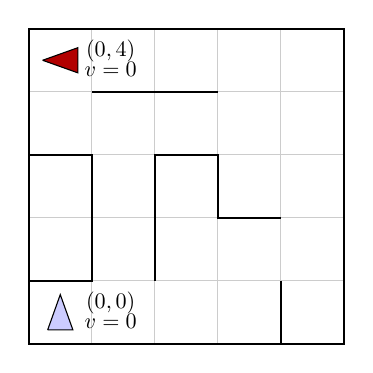
\begin{tikzpicture}[scale=0.8]
    \draw[step=1,gray!40!white,thin] (0,0) grid (5,5);
    \draw[black, thick] (0,0) rectangle (5,5);
    
    \draw[fill=blue!20!white] (0.3, 0.22) -- (0.7, 0.22) -- (0.5, 0.78) -- (0.3, 0.22);
    \draw[fill=red!70!black] (0.22, 4.5) -- (0.78, 4.3) -- (0.78, 4.7) -- (0.22, 4.5);
    \draw[black, thick] (1, 4) -- (3, 4);
    \draw[black, thick] (0, 1) -- (1, 1) -- (1, 3) -- (0, 3);
    \draw[black, thick] (2, 1) -- (2, 3) -- (3, 3) -- (3, 2) -- (4, 2);
    \draw[black, thick] (4, 0) -- (4, 1);

    \node[scale=0.8] at (1.3, 0.65) {$(0, 0)$};
    \node[scale=0.8] at (1.3, 0.35) {$v = 0$};
    \node[scale=0.8] at (1.3, 4.65) {$(0, 4)$};
    \node[scale=0.8] at (1.3, 4.35) {$v = 0$};
    \end{tikzpicture}
\end{center}

Consider a car-like agent trying to navigate out of a maze, similar to the one depicted above. The agent is directional and always faces a specific direction \(d \in (N, S, E, W)\). With each action, the agent has the option to either move forward at a variable speed \(v\) or to turn.

The movement actions include \textit{faster}, \textit{maintain}, and \textit{slower}. When the agent performs these actions, it moves a number of squares corresponding to its \textbf{new} adjusted velocity. Let \(v\) represent the agent's current velocity, and \(v'\) denote the new adjusted velocity.

\begin{itemize}[noitemsep,topsep=0pt]\vspace{-0.3cm}
    \item \textit{Faster}: $v'$ = $v$ + 1
    \item \textit{Slower}: $v'$ = $v$ - 1
    \item \textit{Maintain}: $v'$ = $v$
\end{itemize}

The turning actions are \textit{left} and \textit{right}, which change the agent’s direction by 90 degrees. \textbf{Turning is only permitted when the velocity is zero.} Turning leaves the speed at zero. 
\begin{itemize}[noitemsep,topsep=0pt]\vspace{-0.3cm}
    \item \textit{Left}: change the agent’s direction by 90 degrees counterclockwise
    \item \textit{Right}: change the agent’s direction by 90 degrees clockwise
\end{itemize}

For example, if the agent is currently on (0, 0) facing north with velocity 0 (as pictured) and wants to get to (2, 0) facing east with velocity 0, the sequence of actions will be: \textit{right, faster, maintain, slower}.

\textbf{Illegal actions} include
\begin{itemize}[noitemsep,topsep=0pt]\vspace{-0.3cm}
    \item Any action that would result in a collision with a wall (i.e. there is a wall between the current position and the position you would be in if you took said action)
    \item Any action that would reduce $v$ below 0 (slowing when v=0) or above a maximum speed $V_{max}$ 
    \item Maintaining a velocity of 0
    \item Turning when velocity $ \neq 0$
\end{itemize}

The agent’s goal is to find a plan which parks it ($v = 0$) in the goal direction on the exit square using as few actions (time steps) as possible. Note that the cost of a path is defined by the number of actions the agent takes.

% \begin{question}[3] Suppose the agent wants to take the leftmost path (i.e., the one that passes through (1,2)) from the start (0,0) facing north to the goal (0,4) facing west. Write down the \textbf{shortest} sequence of actions for it to take. 

% \solutionspace{2cm}{15cm}{Actions:}{\Onea}

% \end{question}
% \pagebreak
\begin{question}[3]
If the grid is M by N and the maximum speed is $V_{max}$, what is the size of the state space? You should assume that all configurations are reachable from the start state.

\solutionspace{2cm}{15cm}{State Space Size:}{\Onea}
\end{question}

\begin{question}[3]
A “child” of a state $s$ is any other state $s'$ reachable via a legal action from state $s$. Is it possible that a state in the state space has no children? If so, give an example of such a state. If not, briefly explain why every state must have at least one child.

\hspace{5mm}
\solution{\emptycircle}{\OnebYes} Yes
\hspace{5mm}
\solution{\emptycircle}{\OnebNo} No

\solutionspace{4cm}{15cm}{Example State or Explanation:}{\Onebreason}

\end{question}

\begin{question}[4] 
What is the maximum branching factor of this problem?
Draw an example state (x, y, orientation, velocity) that has this branching factor, and list the set of available actions. For example, in the above picture, if the agent was in (0, 0) facing North with a velocity of $v = 0$, the branching factor would be 2. The agent could turn left or right (but not go faster since it would hit a wall).

Illegal actions are simply not returned by the problem model and therefore not counted in the branching factor. You do not necessarily have to use the example grid above. If you need to include a drawing of your own, label properly and \textbf{make sure it fits in the solution box}.

\solutionspace{1.5cm}{10cm}{Maximum Branching Factor:}{\Onecmax}

\solutionspace{6cm}{15cm}{Maximum Branching Example State and Available Actions:}{\Onecmaxexample}

\end{question}


 
\begin{question}[4]
Is the Manhattan distance from the agent’s location to the exit’s location admissible?

If not, draw an example state (x, y, orientation, velocity) where this heuristic overestimates at that state, and specify: 1) the heuristic value at that state and 2) the actual cost from that state to the goal.

You do not necessarily have to use the example grid above. Make sure to label your drawing, including the goal state (location, orientation, speed) and action sequence, and fit it into the solution box.

\hspace{5mm}
\solution{\emptycircle}{\OnedYes} Yes
\hspace{5mm}
\solution{\emptycircle}{\OnedNo} No

\solutionspace{4cm}{15cm}{Example State, Heuristic Value, Actual Cost: }{\Onedreason}

\end{question}

\begin{question}[4]
Is the following heuristic admissible? \textit{Manhattan distance / $V_{max}$}.

If yes, state why. If not, draw an example state (x, y, orientation, velocity) where this heuristic overestimates at that state, and specify: 1) the heuristic value at that state and 2) the actual cost from that state to the goal.

You do not necessarily have to use the example grid above. Make sure to label your drawing, including the goal state (location, orientation, speed) and action sequence, and fit it into the solution box.

\hspace{5mm}
\solution{\emptycircle}{\OneeYes} Yes
\hspace{5mm}
\solution{\emptycircle}{\OneeNo} No

\solutionspace{6cm}{15cm}{Example State, Heuristic Value, Actual Cost:}{\Oneereason }
\end{question}

\begin{question}[1]
If we used an inadmissible heuristic in A* Tree search, could it change the completeness of the search? Assume the graph is finite and the heuristic is non-negative.

\hspace{5mm}
\solution{\emptycircle}{\OnefYes} Yes
\hspace{5mm}
\solution{\emptycircle}{\OnefNo} No

\solution{}{\Onefreason}
\end{question}

\begin{question}[1]
If we used an inadmissible heuristic in A* Tree search, could it change the optimality of the search? Assume the graph is finite and the heuristic is non-negative.

\hspace{5mm}
\solution{\emptycircle}{\OnegYes} Yes
\hspace{5mm}
\solution{\emptycircle}{\OnegNo} No

\solution{}{\Onegreason}
\end{question}



\begin{question}[3]
Which of the following may be a good reason to use an inadmissible heuristic over an admissible one? \\Select all that apply.

% \hspace{5mm}
\solution{\emptysquare}{\OnehA} An inadmissible heuristic may be easier to compute, leading to a faster state heuristic computation time. \\


% \hspace{5mm}
\solution{\emptysquare}{\OnehB} An inadmissible heuristic can be a closer estimate to the actual cost (even if it’s an overestimate) than an admissible heuristic, thus exploring fewer nodes. \\

% \hspace{5mm}
\solution{\emptysquare}{\OnehC} An inadmissible heuristic will still find optimal paths when the actual costs are non-negative. \\

% \hspace{5mm}
\solution{\emptysquare}{\OnehD} An inadmissible heuristic may be used to completely block off searching part of a graph in a search algorithm.

\solution{}{\OneIReason} 
\end{question}

\end{problem}


\newpage
\newcommand{\inlineq}[1]{$\displaystyle{#1}$}

\begin{problem}{All Searches Lead to the Same Destination}

{\bf For all the questions below assume :}
\begin{itemize}
\item All search algorithms are \emph{graph} search (as opposed to
  tree search).
\item $c_{ij} > 0$ is the cost to go from node $i$ to node $j$.
\item There is only one goal node (as opposed to a set of goal nodes).
\item All ties are broken alphabetically.
\item Assume heuristics are consistent.
\end{itemize}


{\bf Definition:} Two search algorithms are defined to be {\bf\emph{equivalent}} if and only if they expand the same nodes in the same order and return the same path.

In this question we study what happens if we run uniform cost
search with action costs $d_{ij}$ that are potentially different from the search problem's actual action costs $c_{ij}$.   Concretely, we will study how this might, or might
not, result in running uniform cost search (with these new
choices of action costs) being equivalent to another search
algorithm. 

\begin{question}[2]
Mark \emph{all} choices for costs $d_{ij}$ that make running {\bf
  Uniform Cost Search} algorithm with these costs $d_{ij}$ 
\emph{equivalent} to running {\bf Breadth-First Search}.  
	\begin{itemize}	
	\item[] \solution{\emptycircle}{\Twoai}  \inlineq{d_{ij} = 0}
	\item[] \solution{\emptycircle}{\Twoaii}  \inlineq{d_{ij} = \alpha}, ${\alpha > 0}$
	\item[]\solution{\emptycircle}{\Twoaiii}  \inlineq{d_{ij} = \alpha}, ${\alpha < 0}$
	\item[]\solution{\emptycircle}{\Twoaiv}  \inlineq{d_{ij} = 1}
	\item[]\solution{\emptycircle}{\Twoav}  \inlineq{d_{ij} = -1}
	\item[]\solution{\emptycircle}{\Twoavi} None of the above
	\end{itemize}\solution{\vspace{1cm}}{}\end{question}
\begin{question}[2]
Mark \emph{all} choices for costs $d_{ij}$ that make running {\bf
  Uniform Cost Search} algorithm with these costs $d_{ij}$ 
\emph{equivalent} to running {\bf Depth-First Search}.
	\begin{itemize}	
	\item[] \solution{\emptycircle}{\Twobi}  \inlineq{d_{ij} = 0}
	\item[] \solution{\emptycircle}{\Twobii}  \inlineq{d_{ij} = \alpha}, ${\alpha > 0}$
	\item[]\solution{\emptycircle}{\Twobiii}  \inlineq{d_{ij} = \alpha}, ${\alpha < 0}$
	\item[]\solution{\emptycircle}{\Twobiv}  \inlineq{d_{ij} = 1}
	\item[]\solution{\emptycircle}{\Twobv}  \inlineq{d_{ij} = -1}
	\item[]\solution{\emptycircle}{\Twobvi} None of the above
	\end{itemize}\solution{\vspace{1cm}}{}\end{question}
\newpage
\begin{question}[2]
Mark \emph{all} choices for costs $d_{ij}$  that make running {\bf
  Uniform Cost Search} algorithm with these costs $d_{ij}$ 
\emph{equivalent} to running {\bf Uniform Cost Search} with the
original costs $c_{ij}$.
	\begin{itemize}
	\item[]\solution{\emptycircle}{\Twoci} $d_{ij} = c_{ij}^2$
	\item[]\solution{\emptycircle}{\Twocii} $d_{ij} = 1/c_{ij}$
	\item[]\solution{\emptycircle}{\Twociii}  $d_{ij} = \alpha\ c_{ij}, \ \ \ \ \ \ \ \alpha > 0$
	\item[]\solution{\emptycircle}{\Twociv} $d_{ij} = c_{ij} + \alpha, \ \ \ \ \ \alpha > 0$
	\item[]\solution{\emptycircle}{\Twocv}  $d_{ij} = \alpha \ c_{ij} + \beta, \ \ \alpha > 0,\ \beta > 0$
	\item[]\solution{\emptycircle}{\Twocvi} None of the above
	\end{itemize} \solution{\vspace{1cm}}{}\end{question}
\begin{question}
Let $h(n)$ be the value of the heuristic function at node $n$.
\begin{subquestion}[2]
Mark \emph{all} choices for costs $d_{ij}$  that make running {\bf
  Uniform Cost Search} algorithm with these costs $d_{ij}$ 
\emph{equivalent} to running {\bf Greedy Search} with the
original costs $c_{ij}$ and heuristic function $h$.
	\begin{itemize}
	\item[]\solution{\emptycircle}{\Twodia}  \inlineq{d_{ij} = h(i) - h(j)}
	\item[]\solution{\emptycircle}{\Twodib}  \inlineq{d_{ij} = h(j) - h(i)}
	\item[]\solution{\emptycircle}{\Twodic}  \inlineq{d_{ij} = \alpha \ h(i), \ \ \ \ \alpha > 0}
	\item[]\solution{\emptycircle}{\Twodid}  \inlineq{d_{ij} = \alpha \ h(j), \ \ \ \ \alpha > 0}
	\item[]\solution{\emptycircle}{\Twodie}  \inlineq{d_{ij} = c_{ij} + h(j) + h(i)}
	\item[]\solution{\emptycircle}{\Twodif} None of the above
	\end{itemize} 
  \solution{\vspace{1cm}}{
    }
\end{subquestion}
\vspace{1cm}
\begin{subquestion}[2]
Mark \emph{all} choices for costs $d_{ij}$  that make running {\bf
  Uniform Cost Search} algorithm with these costs $d_{ij}$ 
\emph{equivalent} to running {\bf A* Search} with the
original costs $c_{ij}$ and heuristic function $h$.
	\begin{itemize}
	\item[]\solution{\emptycircle}{\Twodiia} \inlineq{d_{ij} = \alpha \ h(i), \ \ \ \alpha > 0}
	\item[]\solution{\emptycircle}{\Twodiib}  \inlineq{d_{ij} = \alpha \ h(j), \ \ \ \alpha > 0}
	\item[]\solution{\emptycircle}{\Twodiic}  \inlineq{d_{ij} = c_{ij} + h(i)}
	\item[]\solution{\emptycircle}{\Twodiid}  \inlineq{d_{ij} = c_{ij} + h(j)}
	\item[]\solution{\emptycircle}{\Twodiie}  \inlineq{d_{ij} = c_{ij} + h(i) - h(j)}
	\item[]\solution{\emptycircle}{\Twodiif}  \inlineq{d_{ij} = c_{ij} + h(j) - h(i)}
	\item[]\solution{\emptycircle}{\Twodiig} None of the above
	\end{itemize} 
  \solution{\vspace{1cm}}{
    
  }
\end{subquestion}
\end{question}
\end{problem}

\newpage
\begin{problem}{Searching a Graph}

\begin{table}[h]
\centering
\begin{minipage}{0.45\linewidth}

\includegraphics[scale=0.3]{figures/graph2.png} 
\end{minipage}
\hspace{1.5cm}
\begin{minipage}{0.45\linewidth}
\begin{tabular}{|l|l|l|}
\hline
Node & $h_1$ & $h_2$\\
\hline
A &12 &11\\
B &6 &7\\
C &9 &6\\
D &3 &4\\
E &3 &5\\
F &2 &1\\
G &0 &0\\
\hline
\end{tabular}
\end{minipage}
\end{table}

Consider the graph shown above. A is the start state and G is the goal state. The costs for each edge are shown on the graph. The graph is bi-directional so each edge can be traversed from either direction. Please refer to the search algorithms \textbf{exactly as presented on the lecture slides} as the ordering of the actions matters.

\begin{question}[15]
For each of the following \textbf{graph search} strategies, mark with an X which (if any) of the listed paths it could return. Note that for some search strategies the specific path returned might depend on tie-breaking behavior. In any such cases, make sure to mark \textbf{all} paths that could be returned under some tie-breaking scheme. If a graph search strategy returns a path not listed, \textbf{write out the correct path} in the \textit{Other} column.\\


\begin{table}[h]
\begin{center}
\begin{tabular}{|l|l|l|l|l|}
\hline
Algorithm & A-C-E-G & A-C-E-F-G & A-B-D-E-F-G & Other\\
\hline
UCS & \begin{minipage}{2cm}~\\(i)\quad\solution{}{\Threeai}~\\~\\\end{minipage} &
\begin{minipage}{2cm}~\\(ii)\quad\solution{}{\Threeaii}~\\~\\\end{minipage} & 
\begin{minipage}{2cm}~\\(iii)\quad\solution{}{\Threeaiii}~\\~\\\end{minipage} &
\begin{minipage}{3cm}~\\(iv)\quad\solution{}{\Threeaiv}~\\~\\\end{minipage}\\

\hline
Greedy with heuristic $h_1$ & \begin{minipage}{2cm}~\\(v)\quad\solution{}{\Threeav}~\\~\\\end{minipage} &
\begin{minipage}{2cm}~\\(vi)\quad\solution{}{\Threeavi}~\\~\\\end{minipage} & 
\begin{minipage}{2cm}~\\(vii)\quad\solution{}{\Threeavii}~\\~\\\end{minipage} &
\begin{minipage}{3cm}~\\(viii)\quad\solution{}{\Threeaviii}~\\~\\\end{minipage}\\

\hline
Greedy with heuristic $h_2$ & \begin{minipage}{2cm}~\\(ix)\quad\solution{}{\Threeaix}~\\~\\\end{minipage} &
\begin{minipage}{2cm}~\\(x)\quad\solution{}{\Threeax}~\\~\\\end{minipage} & 
\begin{minipage}{2cm}~\\(xi)\quad\solution{}{\Threeaxi}~\\~\\\end{minipage} &
\begin{minipage}{3cm}~\\(xii)\quad\solution{}{\Threeaxii}~\\~\\\end{minipage}\\

\hline
A* with heuristic $h_1$ & \begin{minipage}{2cm}~\\(xiii)\quad\solution{}{\Threeaxiii}~\\~\\\end{minipage} &
\begin{minipage}{2cm}~\\(xiv)\quad\solution{}{\Threeaxiv}~\\~\\\end{minipage} & 
\begin{minipage}{2cm}~\\(xv)\quad\solution{}{\Threeaxv}~\\~\\\end{minipage} &
\begin{minipage}{3cm}~\\(xvi)\quad\solution{}{\Threeaxvi}~\\~\\\end{minipage}\\

\hline
A* with heuristic $h_2$ & \begin{minipage}{2cm}~\\(xvii)\quad\solution{}{\Threeaxvii}~\\~\\\end{minipage} &
\begin{minipage}{2cm}~\\(xviii)\quad\solution{}{\Threeaxviii}~\\~\\\end{minipage} & 
\begin{minipage}{2cm}~\\(xix)\quad\solution{}{\Threeaxix}~\\~\\\end{minipage} &
\begin{minipage}{3cm}~\\(xx)\quad\solution{}{\Threeaxx}~\\~\\\end{minipage}\\

\hline
\end{tabular}
\end{center}
\end{table}
  
\end{question}

\begin{question}[2]
What is the cost of the optimal path for uniform cost search from A to G?

\solutionspace{1.2cm}{7.5cm}{Answer:}{ \Threeb}

\end{question}

\begin{question}[4]
Is $h_1$ admissible? Is it consistent?

Admissible: \hspace{5mm}
\solution{\emptycircle}{\ThreeCAdmissibleYes} Yes
\hspace{5mm}
\solution{\emptycircle}{\ThreeCAdmissibleNo} No

\solution{}{\ThreeCAdmissibleReason}

Consistent: \hspace{5mm}
\solution{\emptycircle}{\ThreeCConsistentYes} Yes
\hspace{5mm}
\solution{\emptycircle}{\ThreeCConsistentNo} No

\solution{}{\ThreeCConsistentReason}

\end{question}

\begin{question}[4]
Is $h_2$ admissible? Is it consistent?

Admissible: \hspace{5mm}
\solution{\emptycircle}{\ThreeDAdmissibleYes} Yes
\hspace{5mm}
\solution{\emptycircle}{\ThreeDAdmissibleNo} No

\solution{}{\ThreeDAdmissibleReason}

Consistent: \hspace{5mm}
\solution{\emptycircle}{\ThreeDConsistentYes} Yes
\hspace{5mm}
\solution{\emptycircle}{\ThreeDConsistentNo} No

\solution{}{\ThreeDConsistentReason}


\end{question}

\end{problem}


\newpage
\usetikzlibrary{shapes}
\begin{problem}{Search: Multiple Choice and Short Answer Questions}

\begin{question}[12]
Consider the following true/false questions with each question worth 2 points. For the following search problems, assume every action has a cost of at least $\epsilon$, with $\epsilon > 0$.  Assume any heuristics used are consistent. 

\vspace{2mm}
\hspace{0.5mm}
Depth-first tree-search on a finite graph is guaranteed to be complete. \\
\solution{\emptycircle}{\FourAATrue} \textbf{True}
\hspace{5mm}
\solution{\emptycircle}{\FourAAFalse} \textbf{False} \\
\solution{}{\FourAAReason}

\vspace{2mm}
\hspace{0.5mm}
Breadth-first tree-search on a finite graph is guaranteed to be complete. \\
\solution{\emptycircle}{\FourABTrue} \textbf{True}
\hspace{5mm}
\solution{\emptycircle}{\FourABFalse} \textbf{False} \\
\solution{}{\FourABReason}

\vspace{2mm}
\hspace{0.5mm}
Iterative deepening tree-search on a finite graph is guaranteed to be complete. \\
\solution{\emptycircle}{\FourACTrue} \textbf{True}
\hspace{5mm}
\solution{\emptycircle}{\FourACFalse} \textbf{False} \\
\solution{}{\FourACReason}

\vspace{2mm}
\hspace{0.5mm}
For all graphs without cycles, graph-search contains a larger frontier than tree-search. \\
\solution{\emptycircle}{\FourADTrue} \textbf{True}
\hspace{5mm}
\solution{\emptycircle}{\FourADFalse} \textbf{False} \\
\solution{}{\FourADReason}

\vspace{2mm}
\hspace{0.5mm}
Iterative deepening graph-search has the time complexity of BFS and the space complexity of DFS. \\
\solution{\emptycircle}{\FourAETrue} \textbf{True}
\hspace{5mm}
\solution{\emptycircle}{\FourAEFalse} \textbf{False} \\
\solution{}{\FourAEReason}

\vspace{2mm}
\hspace{0.5mm}
If $h_{1}$(s) is a consistent heuristic and $h_{2}$(s) is a consistent heuristic, then min($h_{1}$(s), $h_{2}$(s)) must be consistent. \\
\solution{\emptycircle}{\FourAFTrue} \textbf{True}
\hspace{5mm}
\solution{\emptycircle}{\FourAFFalse} \textbf{False} \\
\solution{}{\FourAFReason}
\end{question} 
\vspace{2mm}

\begin{question}[5] 
Consider the state space graph shown below. S is the start state and G is the goal state. The costs for each edge are shown on the graph. For the following table below, fill in potential heuristic values such that the heuristic is admissible but not consistent. 

\vspace{10mm}
\begin{centering} 
\hspace{10mm}
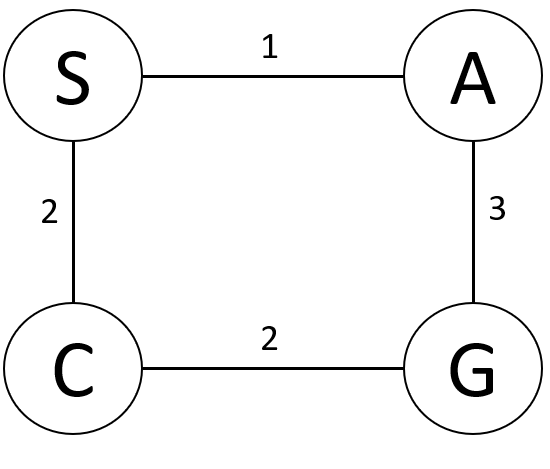
\includegraphics[scale=.6]{figures/Consistent.png} 
\hspace{32mm}{\raisebox{32mm}{
\begin{tabular}{ |p{1.8cm}|p{1.2cm}|  }
\hline
\multicolumn{2}{|c|}{\textbf{Heuristic Function}} \\
\hline
\textbf{State} & \textbf{$h(s)$}  \\
\hline
$S$ & \solution{}{\FourBS}  \\
\hline
$A$ & \solution{}{\FourBA}  \\
\hline
$C$ & \solution{}{\FourBC}   \\
\hline
$G$ &  0 \\
\hline
\end{tabular}}}
\end{centering}

\solution{}{\FourBReason}

\end{question}

\end{problem}
\newpage

\begin{problem}{Search Again}

Consider the state space graph shown below.  A is the start state and
G is the goal state. The costs for each edge are shown on the graph.
Each edge can be traversed in both directions.

\begin{center}
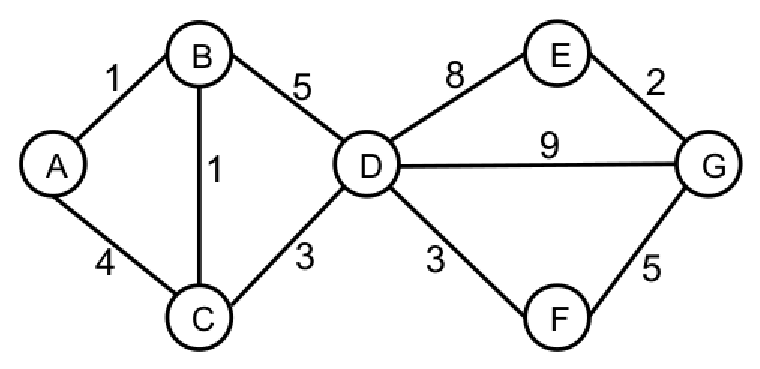
\includegraphics[width=3.5in]{figures/search_graph.eps}
\end{center}

\textbf{Use the Graph Search Algorithm (v2) discussed in class.}
Execute the following search algorithms using priority queues, by
filling in the search table for each part. Write nodes as a tuple containing a state sequence and cost (e.g. (A-B-C, 2)). Note that for Breadth first and Depth first the algorithms ignore the true "cost" so you can just use the depth of the node as the second part of the tuple and then expand nodes with either the highest or lowest depth. Break ties alphabetically.  Note that all steps in the table below will not
necessarily be used. You may skip any steps where a node is removed from the frontier but not expanded. Note that nodes are only expanded after they are removed from the frontier, after checking the goal test, and after checking if not in the closed set.

    
\begin{question}[3]
Breadth First Graph Search

    \begin{tabular}{|l|l@{\hspace*{4.5in}}|l|} \hline
    \bf Step & \bf Priority Queue                                   & \bf Expand \\ \hline
    1 &      \fiveai                                                       & \fiveaib \\ \hline
    2 &     \fiveaii                                                            & \fiveaiib \\ \hline
    3 &    \fiveaiii                                                         & \fiveaiiib \\ \hline
    4 &    \fiveaiv                                                         & \fiveaivb \\ \hline
    5 &      \fiveav                                                       &  \\ \hline
    6 &   \fiveavi                                                          & \fiveavib \\ \hline
    7 &    \fiveavii                                                         & \fiveaviib \\ \hline
    8 &   \fiveaviii                                                          & \fiveaviiib \\ \hline
    \end{tabular}

    Solution: \fivea

\end{question}

\begin{question}[3]
Depth First Graph Search.\\
    \begin{tabular}{|l|l@{\hspace*{4.5in}}|l|} \hline
    \bf Step & \bf Priority Queue                                   & \bf Expand \\ \hline
    1 &      \fivebi                                                       & \fivebib \\ \hline
    2 &     \fivebii                                                            & \fivebiib \\ \hline
    3 &    \fivebiii                                                         & \fivebiiib \\ \hline
    4 &    \fivebiv                                                         & \fivebivb \\ \hline
    5 &      \fivebv                                                       &  \\ \hline
    6 &   \fivebvi                                                          & \fivebvib \\ \hline
    7 &    \fivebvii                                                         & \fivebviib \\ \hline
    8 &   \fivebviii                                                          & \fivebviiib \\ \hline
    \end{tabular}

    Solution:\fiveb
\end{question}

\newpage
\begin{question}[3] 
Uniform Cost Graph Search. \\

    \begin{tabular}{|l|l@{\hspace*{4.5in}}|l|} \hline
    \bf Step & \bf Priority Queue                                   & \bf Expand \\ \hline
    1 &      \fiveci                                                       & \fivecib \\ \hline
    2 &     \fivecii                                                            & \fiveciib \\ \hline
    3 &    \fiveciii                                                         & \fiveciiib \\ \hline
    4 &    \fiveciv                                                         & \fivecivb \\ \hline
    5 &      \fivecv                                                       &  \\ \hline
    6 &   \fivecvi                                                          & \fivecvib \\ \hline
    7 &    \fivecvii                                                         & \fivecviib \\ \hline
    8 &   \fivecviii                                                          & \fivecviiib \\ \hline
    \end{tabular}

    Solution:\fivec


\end{question}

\begin{question}
Heuristic Search

 \begin{subquestion}[4] Consider the two heurisitics $h_1$ and $h_2$, only one of
     which is consistent.  Which one is consistent?

     \fivedh

\end{subquestion}

\begin{center}
\begin{tabular}{|c|c|c|c|c|c|c|c|}\hline
Node  & A   & B  & C  & D  & E   & F   & G  \\ \hline
$h_1$ & 9.5 & 9	 & 8  & 7  & 1.5 & 4   & 0  \\ \hline
$h_2$ & 10  & 12 & 10 & 8  & 1   & 4.5 & 0  \\ \hline
\end{tabular}
\end{center}
\begin{subquestion}[3]
Then do A* search with that heuristic.

    \begin{tabular}{|l|l@{\hspace*{4.5in}}|l|} \hline
    \bf Step & \bf Priority Queue                                   & \bf Expand \\ \hline
    1 &      \fivedi                                                       & \fivedib \\ \hline
    2 &     \fivedii                                                            & \fivediib \\ \hline
    3 &    \fivediii                                                         & \fivediiib \\ \hline
    4 &    \fivediv                                                         & \fivedivb \\ \hline
    5 &      \fivedv                                                       &  \\ \hline
    6 &   \fivedvi                                                          & \fivedvib \\ \hline
    7 &    \fivedvii                                                         & \fivedviib \\ \hline
    8 &   \fivedviii                                                          & \fivedviiib \\ \hline
    \end{tabular}

    Solution: \fived
\end{subquestion}

 \begin{subquestion}[9]
 Suppose you are completing the new heuristic function $h_3$
    shown below.  All the values are fixed except $h_3(B)$.

\begin{center}
\begin{tabular}{|c|c|c|c|c|c|c|c|}
\hline
Node & A & B & C & D & E & F & G \\
\hline
$h_3$& 10 & ?  & 9 & 7 & 1.5 & 4.5& 0 \\
\hline
\end{tabular}
\end{center}

For each of the following conditions, write the set of values that are
possible for $h_3(B)$.  For example, to denote all non-negative
numbers, write [0, $\infty$], to denote the empty set, write
$\emptyset$, and so on.

\begin{enumerate}

\item What values of $h_3(B)$ make $h_3$ admissible?

\fivelasta

\item What values of $h_3(B)$ make $h_3$ consistent?


\fivelastb

\item What values of $h_3(B)$ will cause A* graph search to expand
  from node A to C, then node A to B, then node A to B to D in that
  order?

\fivelastc

\end{enumerate}

\end{subquestion}

\end{question}

\end{problem}
% \newpage
% \input{q6}
\end{document}
